\documentclass[a4paper,9pt,twocolumn,twoside,printwatermark=false]{pinp}

%% Some pieces required from the pandoc template
\providecommand{\tightlist}{%
  \setlength{\itemsep}{0pt}\setlength{\parskip}{0pt}}

% Use the lineno option to display guide line numbers if required.
% Note that the use of elements such as single-column equations
% may affect the guide line number alignment.

\usepackage[T1]{fontenc}
\usepackage[utf8]{inputenc}

% The geometry package layout settings need to be set here...
\geometry{layoutsize={0.95588\paperwidth,0.98864\paperheight},%
          layouthoffset=0.02206\paperwidth,%
		  layoutvoffset=0.00568\paperheight}

\definecolor{pinpblue}{HTML}{185FAF}  % imagecolorpicker on blue for new R logo
\definecolor{pnasbluetext}{RGB}{101,0,0} %



\title{Getting Started in R}

\author[]{Saghir Bashir}


\setcounter{secnumdepth}{3}

% Please give the surname of the lead author for the running footer
\leadauthor{\href{https://creativecommons.org/licenses/by-sa/4.0/}{CC BY SA} ilustat
-- \href{mailto:info@ilustat.com}{\nolinkurl{info@ilustat.com}}}

% Keywords are not mandatory, but authors are strongly encouraged to provide them. If provided, please include two to five keywords, separated by the pipe symbol, e.g:
 \keywords{  R |  Tiyverse |  Statistics |  Data Science  }  

\begin{abstract}
Are you curious to learn what R can do for you? Do you want to see how
it works? If so, then this ``Getting Started'' guide is for you which
introduces you to some key concepts using realistic examples. Using a
real life dataset, it will also show you how to produce graphs and
summary statistics using the ``tidyverse'' package.
\end{abstract}

\dates{This version was compiled on \today}
\doi{\url{http://ilustat.com/}}

\pinpfootercontents{Getting Started in R}

\begin{document}

% Optional adjustment to line up main text (after abstract) of first page with line numbers, when using both lineno and twocolumn options.
% You should only change this length when you've finalised the article contents.
\verticaladjustment{-2pt}

\maketitle
\thispagestyle{firststyle}
\ifthenelse{\boolean{shortarticle}}{\ifthenelse{\boolean{singlecolumn}}{\abscontentformatted}{\abscontent}}{}

% If your first paragraph (i.e. with the \dropcap) contains a list environment (quote, quotation, theorem, definition, enumerate, itemize...), the line after the list may have some extra indentation. If this is the case, add \parshape=0 to the end of the list environment.

\acknow{{[}Names{]} for reviewing the draft versions of this document.}

\section{Preface}\label{preface}

This ``Getting Started'' guide will give you a flavour of what
R\footnote{R project: \url{https://www.r-project.org/}} and the
tidyverse can do for you. To get the most out of this guide, read it
whilst doing the examples and exercises using RStudio\footnote{RStudio
  IDE: \url{https://www.rstudio.com/products/RStudio/}}\^{}.

\subsection{Experiment Safely}\label{experiment-safely}

Be brave and experiment with commands and options as it is an essential
part of the learning process. Things can (and will) go ``wrong'', like,
getting error messages or deleting things that you created from using
this guide. You can recover from most situations (e.g.~by restarting R).
To do this ``safely'' start with a \emph{fresh} R session without any
other data loaded (otherwise you could lose it).

\section{Introduction}\label{introduction}

\subsection{Before Starting}\label{before-starting}

Make sure that you have:

\begin{enumerate}
\def\labelenumi{\arabic{enumi}.}
\tightlist
\item
  R and RStudio installed
\item
  Files downloaded from: \url{https://ilustat.com/resources/}
  \textbf{{[}UPDATE{]}}
\item
  Double click on the file \texttt{"GettingStartedinR.Rproj"} which will
  open RStudio automatically with the right set up to work through this
  guide.
\end{enumerate}

\subsection{Starting R \& RStudio}\label{starting-r-rstudio}

R starts automatically when you open RStudio (see Figure
\ref{fig:rstudio}). The console starts with information about the
version number, license and contributors. The last line is a standard
prompt ``\texttt{\textgreater{}}'' that indicates R is ready and
expecting instructions to do something.

\begin{figure}[H]

{\centering 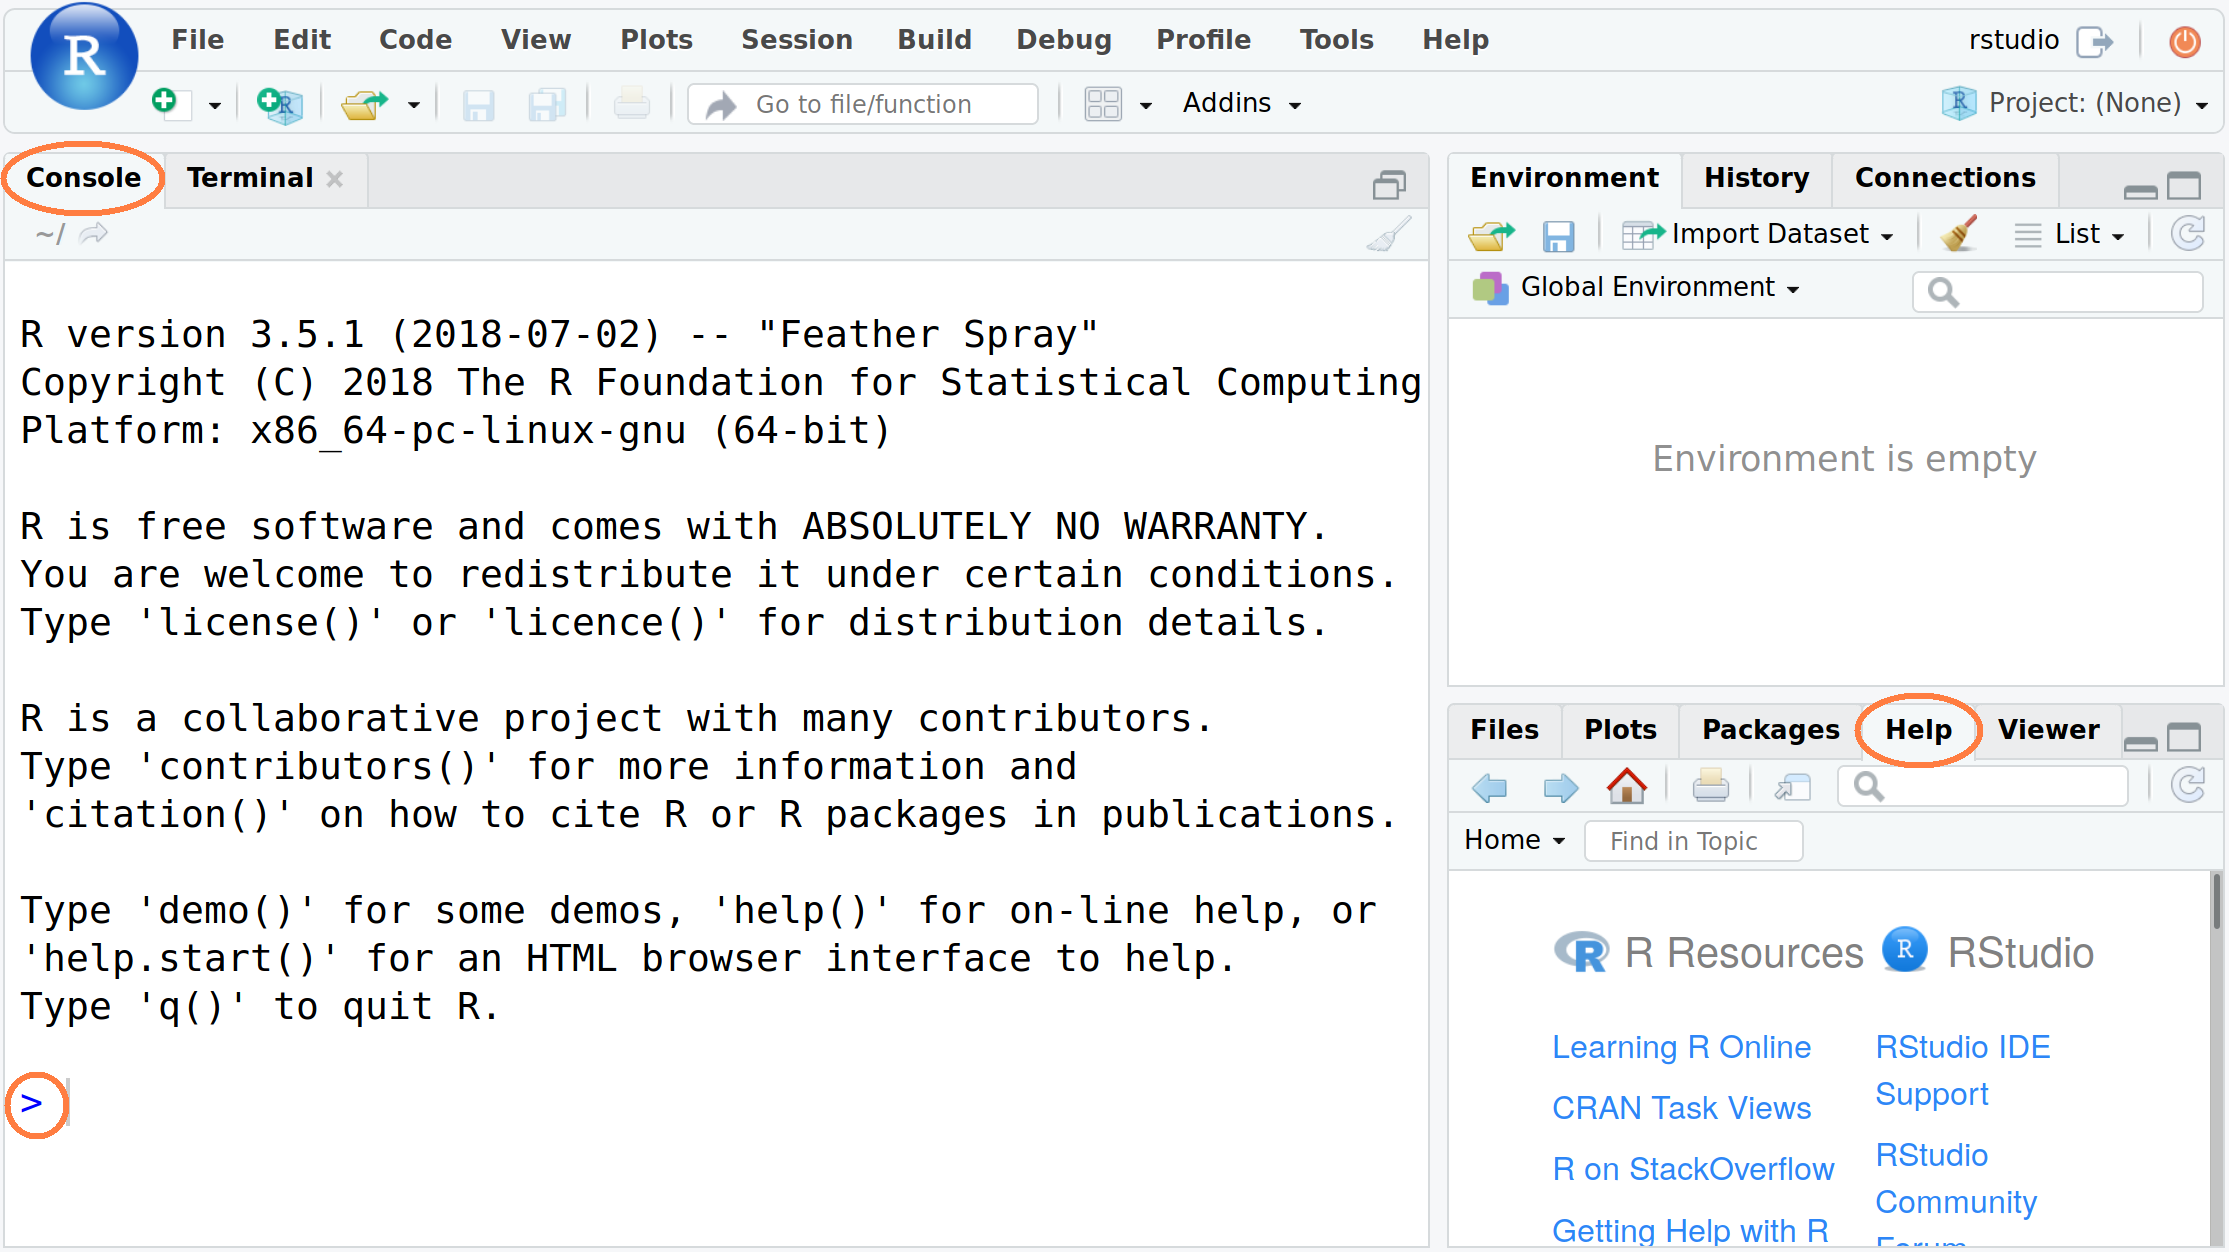
\includegraphics[width=3.4in]{RStudio-Screenshot} 

}

\caption{\label{fig:rstudio}RStudio Screenshot with Console on the left and  Help tab in the bottom right}\label{fig:RStudioScreenshot}
\end{figure}

\subsection{Quitting R \& RStudio}\label{quitting-r-rstudio}

When you quit RStudio you will be asked whether to
\texttt{Save\ workspace} with two options:

\begin{itemize}
\tightlist
\item
  ``Yes'' -- Your current R workspace (containing the work that you have
  done) will be restored next time you open RStudio.
\item
  ``No'' -- You will start with a fresh R session next time you open
  RStudio. For now select ``\emph{No}'' to prevent errors being carried
  over from previous sessions).
\end{itemize}

\section{R Help}\label{r-help}

I strongly recommend that you learn how to use R's useful and extensive
built-in help system as it is an essential part of finding solutions to
your R programming problems. The easiest way is to use RStudio's
``Help'' tab which has a search box (see Figure \ref{fig:rstudio}).

\subsection{\texorpdfstring{\texttt{help()}
function}{help() function}}\label{help-function}

From the R ``Console'' you can use the \texttt{help()} function or
\texttt{?}. For example, try the following two commands (which give the
same result):

\begin{Shaded}
\begin{Highlighting}[]
\KeywordTok{help}\NormalTok{(mean)}
\NormalTok{?mean}
\end{Highlighting}
\end{Shaded}

\subsection{Keyword search}\label{keyword-search}

To do a keyword search use the function \texttt{apropos()} with the
keyword in double quotes (\texttt{"keyword"}) or single quote
(\texttt{\textquotesingle{}keyword\textquotesingle{}}). For example:

\begin{Shaded}
\begin{Highlighting}[]
\KeywordTok{apropos}\NormalTok{(}\StringTok{"mean"}\NormalTok{)}
\end{Highlighting}
\end{Shaded}

\begin{ShadedResult}
\begin{verbatim}
#   [1] ".colMeans"      ".rowMeans"     
#   [3] "colMeans"       "cummean"       
#   [5] "kmeans"         "mean"          
#   [7] "mean_cl_boot"   "mean_cl_normal"
#   [9] "mean_sdl"       "mean_se"       
#  [11] "mean.Date"      "mean.default"  
#  [13] "mean.difftime"  "mean.POSIXct"  
#  [15] "mean.POSIXlt"   "rowMeans"      
#  [17] "weighted.mean"
\end{verbatim}
\end{ShadedResult}

\subsection{Help Examples}\label{help-examples}

Use the \texttt{example()} function to run the examples at the end of
the help for a function:

\begin{Shaded}
\begin{Highlighting}[]
\KeywordTok{example}\NormalTok{(mean)}
\end{Highlighting}
\end{Shaded}

\begin{ShadedResult}
\begin{verbatim}
#  
#  mean> x <- c(0:10, 50)
#  
#  mean> xm <- mean(x)
#  
#  mean> c(xm, mean(x, trim = 0.10))
#  [1] 8.75 5.50
\end{verbatim}
\end{ShadedResult}

\subsection{Searching On-line For R
Help}\label{searching-on-line-for-r-help}

There are a lot of on-line resources that can help. However you must
understand that blindly copying and pasting could be harmful and further
it won't help you to learn and develop. When you search on-line use
\texttt{{[}R{]}} in your search term (e.g.
``\texttt{{[}R{]}\ summary\ \ statistics\ by\ group}''). Note that often
there is more than one solution to your problem. It is good to
investigate the different options.

\subsection{Exercise}\label{exercise}

Try the following:

\begin{itemize}
\tightlist
\item
  \texttt{help(median)}
\item
  \texttt{?sd}
\item
  \texttt{help(unique)}
\end{itemize}

\section{Some R Concepts}\label{some-r-concepts}

In R speak, scalars, vectors/variables and datasets are called
\textbf{\emph{objects}}. To create objects (things) we have to use the
assignment operator ``\texttt{\textless{}-}''. For example, below,
object \texttt{height} is assigned a value of 173 (type \texttt{height}
shows its value):

\begin{Shaded}
\begin{Highlighting}[]
\NormalTok{height <-}\StringTok{ }\DecValTok{173}
\NormalTok{height}
\end{Highlighting}
\end{Shaded}

\begin{ShadedResult}
\begin{verbatim}
#  [1] 173
\end{verbatim}
\end{ShadedResult}

\subsection{Warning: R is case
sensitive}\label{warning-r-is-case-sensitive}

\texttt{age} and \texttt{AGE} are different:

\begin{Shaded}
\begin{Highlighting}[]
\NormalTok{age <-}\StringTok{ }\DecValTok{10}
\NormalTok{AGE <-}\StringTok{ }\DecValTok{50}
\end{Highlighting}
\end{Shaded}

\begin{Shaded}
\begin{Highlighting}[]
\NormalTok{age}
\end{Highlighting}
\end{Shaded}

\begin{ShadedResult}
\begin{verbatim}
#  [1] 10
\end{verbatim}
\end{ShadedResult}

\begin{Shaded}
\begin{Highlighting}[]
\NormalTok{AGE}
\end{Highlighting}
\end{Shaded}

\begin{ShadedResult}
\begin{verbatim}
#  [1] 50
\end{verbatim}
\end{ShadedResult}

\subsection{New lines}\label{new-lines}

R commands are usually separated by a new line but they can also be
separated by a semicolon ``\texttt{;}''.

\begin{Shaded}
\begin{Highlighting}[]
\NormalTok{Name <-}\StringTok{ "Leo"}\NormalTok{; Age <-}\StringTok{ }\DecValTok{25}\NormalTok{; City <-}\StringTok{ "Lisbon"}
\NormalTok{Name; Age; City}
\end{Highlighting}
\end{Shaded}

\begin{ShadedResult}
\begin{verbatim}
#  [1] "Leo"
\end{verbatim}
\end{ShadedResult}\begin{ShadedResult}
\begin{verbatim}
#  [1] 25
\end{verbatim}
\end{ShadedResult}\begin{ShadedResult}
\begin{verbatim}
#  [1] "Lisbon"
\end{verbatim}
\end{ShadedResult}

\subsection{Comments}\label{comments}

It is useful to put human readable comments in your programs. These
comments could help the future you when you go back to your program. R
comments start with a hash sign (\texttt{\#}). Everything after the hash
to the end of the line will be ignored by R.

\begin{Shaded}
\begin{Highlighting}[]
\CommentTok{# This comment line will be ignored when run.}
\NormalTok{AGE       }\CommentTok{# Text after "#" is ignored.}
\end{Highlighting}
\end{Shaded}

\begin{ShadedResult}
\begin{verbatim}
#  [1] 50
\end{verbatim}
\end{ShadedResult}

\subsection{Warning}\label{warning}

If an R command is not complete then R will show a plus sign
(``\texttt{+}'') prompt on second and subsequent lines until the command
syntax is correct.

\begin{Shaded}
\begin{Highlighting}[]
\OperatorTok{+}
\end{Highlighting}
\end{Shaded}

To break out this, press the escape key (\texttt{ESC}).

\subsection{Recalling previous
commands}\label{recalling-previous-commands}

To recall a previously typed commands use the up arrow key
(\(\uparrow\)). To go between previously typed commands use the up and
down arrow (\(\downarrow\)) keys. Once a command is recalled, it can be
modified/corrected using the left (\(\leftarrow\)) and right arrow
(\(\rightarrow\)) keys.

\section{R as a Calculator}\label{r-as-a-calculator}

You can use R as a calculator. Try the following:

\begin{Shaded}
\begin{Highlighting}[]
\DecValTok{2} \OperatorTok{+}\StringTok{ }\DecValTok{3}           
\end{Highlighting}
\end{Shaded}

\begin{ShadedResult}
\begin{verbatim}
#  [1] 5
\end{verbatim}
\end{ShadedResult}

\begin{Shaded}
\begin{Highlighting}[]
\NormalTok{(}\DecValTok{5}\OperatorTok{*}\DecValTok{11}\NormalTok{)}\OperatorTok{/}\DecValTok{4} \OperatorTok{-}\StringTok{ }\DecValTok{7}     
\end{Highlighting}
\end{Shaded}

\begin{ShadedResult}
\begin{verbatim}
#  [1] 6.75
\end{verbatim}
\end{ShadedResult}

\begin{Shaded}
\begin{Highlighting}[]
\CommentTok{# ^ = "to the power of"}
\DecValTok{7}\OperatorTok{^}\DecValTok{3} 
\end{Highlighting}
\end{Shaded}

\begin{ShadedResult}
\begin{verbatim}
#  [1] 343
\end{verbatim}
\end{ShadedResult}

\subsection{Other math functions}\label{other-math-functions}

You can also use standard mathematical functions that are typically
found on a scientific calculator.

\begin{itemize}
\tightlist
\item
  Trigonometric: \texttt{sin()}, \texttt{cos()}, \texttt{tan()},
  \texttt{acos()}, \texttt{asin()}, \texttt{atan()}
\item
  Rounding: \texttt{abs()}, \texttt{ceiling()}, \texttt{floor()},
  \texttt{round()}, \texttt{sign()}, \texttt{signif()}, \texttt{sqrt()},
  \texttt{trunc()}
\item
  Logarithms \& Exponentials: \texttt{exp()}, \texttt{log()},
  \texttt{log10()}, \texttt{log2()}
\end{itemize}

\begin{Shaded}
\begin{Highlighting}[]
\CommentTok{# Square root}
\KeywordTok{sqrt}\NormalTok{(}\DecValTok{2}\NormalTok{)          }
\end{Highlighting}
\end{Shaded}

\begin{ShadedResult}
\begin{verbatim}
#  [1] 1.414214
\end{verbatim}
\end{ShadedResult}

\begin{Shaded}
\begin{Highlighting}[]
\CommentTok{# Round down to nearest integer}
\KeywordTok{floor}\NormalTok{(}\FloatTok{8.6178}\NormalTok{)}
\end{Highlighting}
\end{Shaded}

\begin{ShadedResult}
\begin{verbatim}
#  [1] 8
\end{verbatim}
\end{ShadedResult}

\begin{Shaded}
\begin{Highlighting}[]
\CommentTok{# Round up to nearest integer}
\KeywordTok{ceiling}\NormalTok{(}\FloatTok{8.6178}\NormalTok{)}
\end{Highlighting}
\end{Shaded}

\begin{ShadedResult}
\begin{verbatim}
#  [1] 9
\end{verbatim}
\end{ShadedResult}

\begin{Shaded}
\begin{Highlighting}[]
\CommentTok{# Round to 2 decimal places}
\KeywordTok{round}\NormalTok{(}\FloatTok{8.6178}\NormalTok{, }\DecValTok{2}\NormalTok{)}
\end{Highlighting}
\end{Shaded}

\begin{ShadedResult}
\begin{verbatim}
#  [1] 8.62
\end{verbatim}
\end{ShadedResult}

\subsection{Exercise}\label{exercise-1}

Try out five of the mathemtical functions above, using the help page
where necessary.

\section{Some More R Concepts}\label{some-more-r-concepts}

You can do some clever and useful things with using the assignment
operator ``\texttt{\textless{}-}'':

\begin{Shaded}
\begin{Highlighting}[]
\NormalTok{roomLength <-}\StringTok{ }\FloatTok{7.8}
\NormalTok{roomWidth <-}\StringTok{ }\FloatTok{6.4}
\NormalTok{roomArea <-}\StringTok{ }\NormalTok{roomLength }\OperatorTok{*}\StringTok{ }\NormalTok{roomWidth}
\NormalTok{roomArea}
\end{Highlighting}
\end{Shaded}

\begin{ShadedResult}
\begin{verbatim}
#  [1] 49.92
\end{verbatim}
\end{ShadedResult}

\subsection{Text objects}\label{text-objects}

You can also assign text to an objects.

\begin{Shaded}
\begin{Highlighting}[]
\NormalTok{Greeting <-}\StringTok{ "Hello World!"}
\NormalTok{Greeting}
\end{Highlighting}
\end{Shaded}

\begin{ShadedResult}
\begin{verbatim}
#  [1] "Hello World!"
\end{verbatim}
\end{ShadedResult}

\subsection{Vectors}\label{vectors}

The objects presented so far have all been scalars (single values).
Working with vectors is where R shines best as they are the basic
building blocks of datasets. To create a vector we can use the
\texttt{c()} (combine values into a vector) function.

\begin{Shaded}
\begin{Highlighting}[]
\CommentTok{# A "numeric" vector}
\NormalTok{x1 <-}\StringTok{ }\KeywordTok{c}\NormalTok{(}\DecValTok{26}\NormalTok{, }\DecValTok{10}\NormalTok{, }\DecValTok{4}\NormalTok{, }\DecValTok{7}\NormalTok{, }\DecValTok{41}\NormalTok{, }\DecValTok{19}\NormalTok{)}
\NormalTok{x1}
\end{Highlighting}
\end{Shaded}

\begin{ShadedResult}
\begin{verbatim}
#  [1] 26 10  4  7 41 19
\end{verbatim}
\end{ShadedResult}

\begin{Shaded}
\begin{Highlighting}[]
\CommentTok{# A "character" vector of country names}
\NormalTok{x2 <-}\StringTok{ }\KeywordTok{c}\NormalTok{(}\StringTok{"Peru"}\NormalTok{, }\StringTok{"Italy"}\NormalTok{, }\StringTok{"Cuba"}\NormalTok{, }\StringTok{"Ghana"}\NormalTok{)  }
\NormalTok{x2}
\end{Highlighting}
\end{Shaded}

\begin{ShadedResult}
\begin{verbatim}
#  [1] "Peru"  "Italy" "Cuba"  "Ghana"
\end{verbatim}
\end{ShadedResult}

There are many other ways to create vectors, for example, \texttt{rep()}
(replicate elements) and \texttt{seq()} (create sequences):

\begin{Shaded}
\begin{Highlighting}[]
\CommentTok{# Repeat vector (2, 6, 7, 4) three times}
\NormalTok{r1 <-}\StringTok{ }\KeywordTok{rep}\NormalTok{(}\KeywordTok{c}\NormalTok{(}\DecValTok{2}\NormalTok{, }\DecValTok{6}\NormalTok{, }\DecValTok{7}\NormalTok{, }\DecValTok{4}\NormalTok{), }\DataTypeTok{times=}\DecValTok{3}\NormalTok{)}
\NormalTok{r1}
\end{Highlighting}
\end{Shaded}

\begin{ShadedResult}
\begin{verbatim}
#   [1] 2 6 7 4 2 6 7 4 2 6 7 4
\end{verbatim}
\end{ShadedResult}

\begin{Shaded}
\begin{Highlighting}[]
\CommentTok{# Vector from -2 to 3 incremented by half}
\NormalTok{s1 <-}\StringTok{ }\KeywordTok{seq}\NormalTok{(}\DataTypeTok{from=}\OperatorTok{-}\DecValTok{2}\NormalTok{, }\DataTypeTok{to=}\DecValTok{3}\NormalTok{, }\DataTypeTok{by=}\FloatTok{0.5}\NormalTok{)}
\NormalTok{s1}
\end{Highlighting}
\end{Shaded}

\begin{ShadedResult}
\begin{verbatim}
#   [1] -2.0 -1.5 -1.0 -0.5  0.0  0.5  1.0  1.5
#   [9]  2.0  2.5  3.0
\end{verbatim}
\end{ShadedResult}

\subsection{Vector operations}\label{vector-operations}

You can do also calculations on vectors, for example using \texttt{x1}
from above:

\begin{Shaded}
\begin{Highlighting}[]
\NormalTok{x1 }\OperatorTok{*}\StringTok{ }\DecValTok{2}
\end{Highlighting}
\end{Shaded}

\begin{ShadedResult}
\begin{verbatim}
#  [1] 52 20  8 14 82 38
\end{verbatim}
\end{ShadedResult}

\begin{Shaded}
\begin{Highlighting}[]
\KeywordTok{round}\NormalTok{(}\KeywordTok{sqrt}\NormalTok{(x1}\OperatorTok{*}\FloatTok{2.6}\NormalTok{), }\DecValTok{2}\NormalTok{)}
\end{Highlighting}
\end{Shaded}

\begin{ShadedResult}
\begin{verbatim}
#  [1]  8.22  5.10  3.22  4.27 10.32  7.03
\end{verbatim}
\end{ShadedResult}

\subsection{Missing Values}\label{missing-values}

Missing values are coded as \texttt{NA} in R. For example,

\begin{Shaded}
\begin{Highlighting}[]
\NormalTok{x2 <-}\StringTok{ }\KeywordTok{c}\NormalTok{(}\DecValTok{3}\NormalTok{, }\OperatorTok{-}\DecValTok{7}\NormalTok{, }\OtherTok{NA}\NormalTok{, }\DecValTok{5}\NormalTok{, }\DecValTok{1}\NormalTok{, }\DecValTok{1}\NormalTok{) }
\NormalTok{x2}
\end{Highlighting}
\end{Shaded}

\begin{ShadedResult}
\begin{verbatim}
#  [1]  3 -7 NA  5  1  1
\end{verbatim}
\end{ShadedResult}

\begin{Shaded}
\begin{Highlighting}[]
\NormalTok{x3 <-}\StringTok{ }\KeywordTok{c}\NormalTok{(}\StringTok{"Rat"}\NormalTok{, }\OtherTok{NA}\NormalTok{, }\StringTok{"Mouse"}\NormalTok{, }\StringTok{"Hamster"}\NormalTok{)}
\NormalTok{x3}
\end{Highlighting}
\end{Shaded}

\begin{ShadedResult}
\begin{verbatim}
#  [1] "Rat"     NA        "Mouse"   "Hamster"
\end{verbatim}
\end{ShadedResult}

\subsection{Managing Objects}\label{managing-objects}

Use function \texttt{ls()} to list the objects in your workspace. The
\texttt{rm()} function removes (delete) them.

\begin{Shaded}
\begin{Highlighting}[]
\KeywordTok{ls}\NormalTok{()}
\end{Highlighting}
\end{Shaded}

\begin{ShadedResult}
\begin{verbatim}
#   [1] "age"        "Age"        "AGE"       
#   [4] "City"       "Greeting"   "height"    
#   [7] "Name"       "r1"         "roomArea"  
#  [10] "roomLength" "roomWidth"  "s1"        
#  [13] "x"          "x1"         "x2"        
#  [16] "x3"         "xm"
\end{verbatim}
\end{ShadedResult}

\begin{Shaded}
\begin{Highlighting}[]
\KeywordTok{rm}\NormalTok{(x, x1, x2, x3, xm, r1, s1, AGE, age)}
\KeywordTok{ls}\NormalTok{()}
\end{Highlighting}
\end{Shaded}

\begin{ShadedResult}
\begin{verbatim}
#  [1] "Age"        "City"       "Greeting"  
#  [4] "height"     "Name"       "roomArea"  
#  [7] "roomLength" "roomWidth"
\end{verbatim}
\end{ShadedResult}

\section{R Functions and Packages}\label{r-functions-and-packages}

\subsection{R Functions}\label{r-functions}

We have already used some R functions (e.g. \texttt{c()},
\texttt{mean()}, \texttt{rep()}, \texttt{sqrt()}, \texttt{round()}).
Most of the computations in R involves using functions. A function
essentially has a name and a list of arguments separated by a comma.
Let's have look at an example:

\begin{Shaded}
\begin{Highlighting}[]
\KeywordTok{seq}\NormalTok{(}\DataTypeTok{from =} \DecValTok{5}\NormalTok{, }\DataTypeTok{to =} \DecValTok{8}\NormalTok{, }\DataTypeTok{by =} \FloatTok{0.4}\NormalTok{)}
\end{Highlighting}
\end{Shaded}

\begin{ShadedResult}
\begin{verbatim}
#  [1] 5.0 5.4 5.8 6.2 6.6 7.0 7.4 7.8
\end{verbatim}
\end{ShadedResult}

The function name is \texttt{seq} and it has three arguments
\texttt{from}, \texttt{to} and \texttt{by}. The arguments \texttt{from}
and \texttt{to} are the start and end values of a sequence that you want
to create, and \texttt{by} is the increment of the sequence. The
\texttt{seq()} functions has other arguments that you could use which
are documented in the help page. For example, we could use the argument
\texttt{length.out} (instead of \texttt{by}) to fix the length of the
sequence as follows:

\begin{Shaded}
\begin{Highlighting}[]
\KeywordTok{seq}\NormalTok{(}\DataTypeTok{from =} \DecValTok{5}\NormalTok{, }\DataTypeTok{to =} \DecValTok{8}\NormalTok{, }\DataTypeTok{length.out =} \DecValTok{16}\NormalTok{)}
\end{Highlighting}
\end{Shaded}

\begin{ShadedResult}
\begin{verbatim}
#   [1] 5.0 5.2 5.4 5.6 5.8 6.0 6.2 6.4 6.6 6.8
#  [11] 7.0 7.2 7.4 7.6 7.8 8.0
\end{verbatim}
\end{ShadedResult}

\subsection{Custom Functions}\label{custom-functions}

You can create your own functions (using the \texttt{function()}
function) which is a very powerful way to extend R. Writing your own
functions is outside the scope of this guide. As you get more and more
familiar with R it is very likely that you will need to learn do so but
for now you don't need to.

\subsection{R Packages}\label{r-packages}

You can do many things with a standard R installation and it can be
extended using contributed packages. Packages are like apps for R. They
can contain functions, data and documentation.

\subsection{\texorpdfstring{\texttt{tidyverse}}{tidyverse}}\label{tidyverse}

The \texttt{tidyverse} package\footnote{Tidyverse:
  \url{https://www.tidyverse.org/}} is a collection of packages the lets
you import, manipulate, explore, visualise and model data in a
harmonised and consistent way which helps you to be more productive. We
will use the \texttt{tidyverse} to visualise and summarise data.

\subsection{\texorpdfstring{To continue please install the
\texttt{tidyverse}
package}{To continue please install the tidyverse package}}\label{to-continue-please-install-the-tidyverse-package}

\begin{Shaded}
\begin{Highlighting}[]
\KeywordTok{install.packages}\NormalTok{(}\StringTok{"tidyverse"}\NormalTok{)}
\end{Highlighting}
\end{Shaded}

\subsection{Loading packages}\label{loading-packages}

To use the \texttt{tidyverse} package load it using the
\texttt{library()} function:

\begin{Shaded}
\begin{Highlighting}[]
\KeywordTok{library}\NormalTok{(tidyverse)}
\end{Highlighting}
\end{Shaded}

\section{Chick Weight Data}\label{chick-weight-data}

R comes with many datasets installed\footnote{Type \texttt{data()} in
  the R console to see a list of the datasets.}. We will use the
\texttt{ChickWeight} dataset to learn about the tidyverse. The help
system gives a basic summary of the experiment from which the data was
collect:

\begin{quote}
\emph{``The body weights of the chicks were measured at birth and every
second day thereafter until day 20. They were also measured on day 21.
There were four groups of chicks on different protein diets.''}
\end{quote}

You can get more information, including references by typing:

\begin{Shaded}
\begin{Highlighting}[]
\KeywordTok{help}\NormalTok{(}\StringTok{"ChickWeight"}\NormalTok{)}
\end{Highlighting}
\end{Shaded}

\subsection{The Data}\label{the-data}

There are 578 observations (rows) and 4 variables:

\begin{itemize}
\tightlist
\item
  \texttt{Chick} -- unique ID for each chick.
\item
  \texttt{Diet} -- one of four protein diets.
\item
  \texttt{Time} -- number of days since birth.
\item
  \texttt{weight} -- body weight of chick in grams.
\end{itemize}

\subsection{Note}\label{note}

\texttt{weight} has a lower case \texttt{w} (recall R is case
sensitive).

\subsection{Objective}\label{objective}

Investigate the \emph{effect of diet on the weight over time}.

\section{Importing The Data}\label{importing-the-data}

First we will import the data from a file called
\texttt{ChickWeight.csv} using the \texttt{read\_csv()} function from
the \texttt{readr} package (part of the \texttt{tidyverse}). The first
thing to do, outside of R, is to open the file \texttt{ChickWeight.csv}
to check what it contains and that it makes sense. Now we can import the
data as follows:

\begin{Shaded}
\begin{Highlighting}[]
\NormalTok{CW <-}\StringTok{ }\KeywordTok{read_csv}\NormalTok{(}\StringTok{"ChickWeight.csv"}\NormalTok{)}
\end{Highlighting}
\end{Shaded}

\begin{ShadedResult}
\begin{verbatim}
#  Parsed with column specification:
#  cols(
#    Chick = col_double(),
#    Diet = col_double(),
#    Time = col_double(),
#    weight = col_double()
#  )
\end{verbatim}
\end{ShadedResult}

All columns (variables) have been read in as numeric values (i.e.
\texttt{col\_double()}) but you may see that they are read in a integer
(i.e. \texttt{col\_int()}) due to operating system differences.

\subsection{Important Note}\label{important-note}

If all goes well then the data is now stored in an R object called
\texttt{CW}. If you get the following error message then you need to
change the working directory to where the data is stored.

\begin{verbatim}
Error: 'ChickWeight.csv' does not exist in current
working directory ...
\end{verbatim}

\subsection{Change the working directory in
RStudio}\label{change-the-working-directory-in-rstudio}

From the menu bar select ``Session - Set Working Directory - Choose
Directory\ldots{}'' then go to the directory where the data is stored.
Alternatively, within in R, you could use the function
\texttt{setwd()}\footnote{Use \texttt{getwd()} to see the current
  working directory and \texttt{setwd("/to/data/path/data.csv")} to
  change it (important to use \texttt{/} even for Microsoft Windows).}.

\section{Looking at the Dataset}\label{looking-at-the-dataset}

To look at the data type just type the object (dataset) name:

\begin{Shaded}
\begin{Highlighting}[]
\NormalTok{CW}
\end{Highlighting}
\end{Shaded}

\begin{ShadedResult}
\begin{verbatim}
#  # A tibble: 578 x 4
#     Chick  Diet  Time weight
#     <dbl> <dbl> <dbl>  <dbl>
#   1    18     1     0     39
#   2    18     1     2     35
#   3    16     1     0     41
#   4    16     1     2     45
#   5    16     1     4     49
#   6    16     1     6     51
#   7    16     1     8     57
#   8    16     1    10     51
#   9    16     1    12     54
#  10    15     1     0     41
#  # ... with 568 more rows
\end{verbatim}
\end{ShadedResult}

\subsection{\texorpdfstring{\texttt{glimpse()}
function}{glimpse() function}}\label{glimpse-function}

If there are too many variables then not all them may be printed. To
overcome this issue we can use the \texttt{glimpse()} function which
makes it possible to see every column in your dataset (called a ``data
frame'' in R speak).

\begin{Shaded}
\begin{Highlighting}[]
\KeywordTok{glimpse}\NormalTok{(CW)}
\end{Highlighting}
\end{Shaded}

\begin{ShadedResult}
\begin{verbatim}
#  Observations: 578
#  Variables: 4
#  $ Chick  <dbl> 18, 18, 16, 16, 16, 16, 1...
#  $ Diet   <dbl> 1, 1, 1, 1, 1, 1, 1, 1, 1...
#  $ Time   <dbl> 0, 2, 0, 2, 4, 6, 8, 10, ...
#  $ weight <dbl> 39, 35, 41, 45, 49, 51, 5...
\end{verbatim}
\end{ShadedResult}

\subsection{Interpretation}\label{interpretation}

Both of these show that the dataset has 578 observations and 4 variables
as we would expect and as compared to the original data file
\texttt{ChicWeight.csv}. So a good start.

\subsection{Exercise}\label{exercise-2}

It is important to look at the last observations of the dataset as it
could reveal potential data issues. Use the \texttt{tail()} function to
do this. Is it consistent with the original data file
\texttt{ChickWeight.csv}?

\section{Chick Weight: Data
Visualisation}\label{chick-weight-data-visualisation}

\subsection{\texorpdfstring{\texttt{ggplot2}
Package}{ggplot2 Package}}\label{ggplot2-package}

To visualise the chick weight data, we will use the \texttt{ggplot2}
package (included in the tidyverse). Our interest is in seeing how the
\emph{weight changes over time for the chicks by diet}. For the moment
don't worry too much about the details just try to build your own
understanding and logic. To learn more try different things even if you
get an error messages.

\subsection{First plot}\label{first-plot}

Let's plot the weight data (vertical axis) over time (horizontal axis).

\begin{Shaded}
\begin{Highlighting}[]
\CommentTok{# An empty plot (the plot on the left)}
\KeywordTok{ggplot}\NormalTok{(CW, }\KeywordTok{aes}\NormalTok{(Time, weight))  }
\CommentTok{# With data (the plot on the right)}
\KeywordTok{ggplot}\NormalTok{(CW, }\KeywordTok{aes}\NormalTok{(Time, weight)) }\OperatorTok{+}\StringTok{ }\KeywordTok{geom_point}\NormalTok{() }
\end{Highlighting}
\end{Shaded}

\begin{center}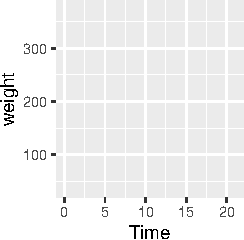
\includegraphics{Getting-Started-in-R_files/figure-latex/emptyPlot-1} 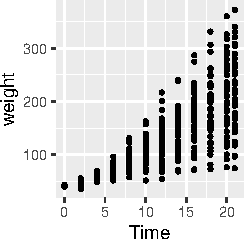
\includegraphics{Getting-Started-in-R_files/figure-latex/emptyPlot-2} \end{center}

\subsection{Exercise}\label{exercise-3}

Switch the variables \texttt{Time} and \texttt{weight} in code used for
the plot on the right? What do you think of this new plot compared to
the original?

\subsection{\texorpdfstring{Add colour for
\texttt{Diet}}{Add colour for Diet}}\label{add-colour-for-diet}

The graph above does not differentiate between the diets. Let's use a
different colour for each diet.

\begin{Shaded}
\begin{Highlighting}[]
\CommentTok{# Adding colour for diet}
\KeywordTok{ggplot}\NormalTok{(CW,}\KeywordTok{aes}\NormalTok{(Time,weight,}\DataTypeTok{colour=}\KeywordTok{factor}\NormalTok{(Diet))) }\OperatorTok{+}
\StringTok{  }\KeywordTok{geom_point}\NormalTok{() }
\end{Highlighting}
\end{Shaded}

\begin{center}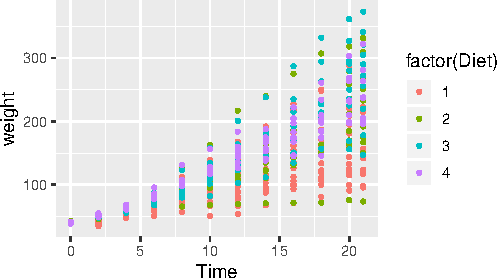
\includegraphics{Getting-Started-in-R_files/figure-latex/addColourPlot-1} \end{center}

\subsection{Interpretation}\label{interpretation-1}

It is difficult to conclude anything from this graph as the points are
printed on top of each other with diet 1 at the bottom and diet 4 on
top.

\subsection{Factor Variables}\label{factor-variables}

Before we continue, we have to make an important change to the
\texttt{CW} dataset by making \texttt{Diet} and \texttt{Time}
\emph{factor variables}. This means that R will treat them as
categorical variables (see the \texttt{\textless{}fct\textgreater{}}
variables below) instead of continuous variables. It will simplify our
coding. The next section will explain the \texttt{mutate()} function.

\begin{Shaded}
\begin{Highlighting}[]
\NormalTok{CW <-}\StringTok{ }\KeywordTok{mutate}\NormalTok{(CW, }\DataTypeTok{Diet =} \KeywordTok{factor}\NormalTok{(Diet))}
\NormalTok{CW <-}\StringTok{ }\KeywordTok{mutate}\NormalTok{(CW, }\DataTypeTok{Time =} \KeywordTok{factor}\NormalTok{(Time))}
\KeywordTok{glimpse}\NormalTok{(CW)}
\end{Highlighting}
\end{Shaded}

\begin{ShadedResult}
\begin{verbatim}
#  Observations: 578
#  Variables: 4
#  $ Chick  <dbl> 18, 18, 16, 16, 16, 16, 1...
#  $ Diet   <fct> 1, 1, 1, 1, 1, 1, 1, 1, 1...
#  $ Time   <fct> 0, 2, 0, 2, 4, 6, 8, 10, ...
#  $ weight <dbl> 39, 35, 41, 45, 49, 51, 5...
\end{verbatim}
\end{ShadedResult}

\subsection{\texorpdfstring{\texttt{facet\_wrap()}
function}{facet\_wrap() function}}\label{facet_wrap-function}

To plot each diet separately in a grid using \texttt{facet\_wrap()}:

\begin{Shaded}
\begin{Highlighting}[]
\CommentTok{# Adding jitter to the points}
\KeywordTok{ggplot}\NormalTok{(CW, }\KeywordTok{aes}\NormalTok{(Time, weight, }\DataTypeTok{colour=}\NormalTok{Diet)) }\OperatorTok{+}
\StringTok{  }\KeywordTok{geom_point}\NormalTok{() }\OperatorTok{+}
\StringTok{  }\KeywordTok{facet_wrap}\NormalTok{(}\OperatorTok{~}\NormalTok{Diet) }\OperatorTok{+}
\StringTok{  }\KeywordTok{theme}\NormalTok{(}\DataTypeTok{legend.position =} \StringTok{"bottom"}\NormalTok{)}
\end{Highlighting}
\end{Shaded}

\begin{center}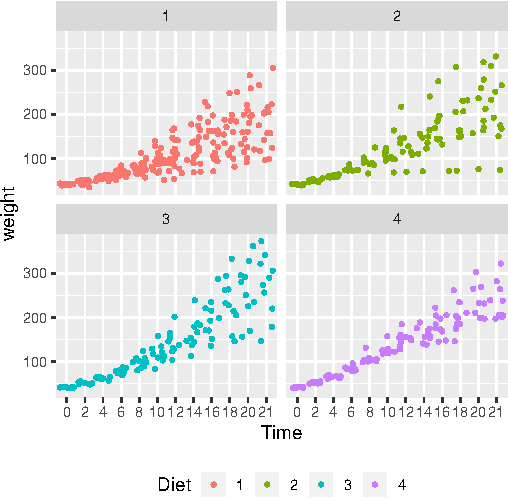
\includegraphics{Getting-Started-in-R_files/figure-latex/jitterPlot-1} \end{center}

\subsection{Exercise}\label{exercise-4}

To overcome the issue of ovelapping points we can \textbf{\emph{jitter}}
the points using \texttt{geom\_jitter()}. Replace the
\texttt{geom\_point()} above with \texttt{geom\_jitter()}.

\subsection{Interpretation}\label{interpretation-2}

Diet 4 has the least variability but we can't really say anything about
the mean effect of each diet.

\subsection{Exercise}\label{exercise-5}

For the \texttt{legend.position} try using ``top'', ``left'' and
``none''. Do we really need a legend for this plot?

\subsection{Mean line plot}\label{mean-line-plot}

Next we will plot the mean changes over time for each diet using the
\texttt{stat\_summary()} function:

\begin{Shaded}
\begin{Highlighting}[]
\KeywordTok{ggplot}\NormalTok{(CW, }\KeywordTok{aes}\NormalTok{(Time, weight, }
               \DataTypeTok{group=}\NormalTok{Diet, }\DataTypeTok{colour=}\NormalTok{Diet)) }\OperatorTok{+}
\StringTok{  }\KeywordTok{stat_summary}\NormalTok{(}\DataTypeTok{fun.y=}\StringTok{"mean"}\NormalTok{, }\DataTypeTok{geom=}\StringTok{"line"}\NormalTok{) }
\end{Highlighting}
\end{Shaded}

\begin{center}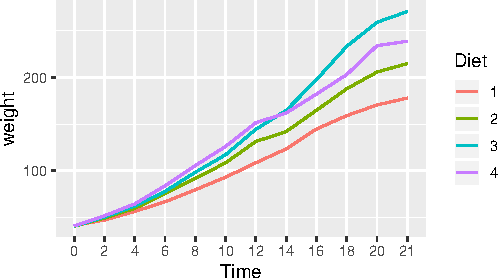
\includegraphics{Getting-Started-in-R_files/figure-latex/meanlinesPlot-1} \end{center}

\subsection{Interpretation}\label{interpretation-3}

This plot is easier to interpret then the previous plots. It shows that
diet 3 group of chicks has the highest mean weight gains by the end of
the experiment. However we don't see the variation (uncertainty) in the
data.

\subsection{Exercise}\label{exercise-6}

What happens when you add \texttt{geom\_point()} to the plot above?
Don't forget the \texttt{+}. Does it make a difference if you put it
before the \texttt{stat\_summary(...)} line? Hint: Look very carefully
at how the graph is plotted.

\subsection{Box-whisker plot}\label{box-whisker-plot}

To see variation between the different diets we use
\texttt{geom\_boxplot} to plot a box-whisker plot. A note caution is
that the number of chicks per diet is relatively low to produce this
plot.

\begin{Shaded}
\begin{Highlighting}[]
\KeywordTok{ggplot}\NormalTok{(CW, }\KeywordTok{aes}\NormalTok{(Time, weight, }\DataTypeTok{colour=}\NormalTok{Diet)) }\OperatorTok{+}
\StringTok{  }\KeywordTok{facet_wrap}\NormalTok{(}\OperatorTok{~}\NormalTok{Diet) }\OperatorTok{+}
\StringTok{  }\KeywordTok{geom_boxplot}\NormalTok{() }\OperatorTok{+}
\StringTok{  }\KeywordTok{theme}\NormalTok{(}\DataTypeTok{legend.position =} \StringTok{"none"}\NormalTok{) }\OperatorTok{+}
\StringTok{  }\KeywordTok{ggtitle}\NormalTok{(}\StringTok{"Chick Weight over Time by Diet"}\NormalTok{)}
\end{Highlighting}
\end{Shaded}

\begin{center}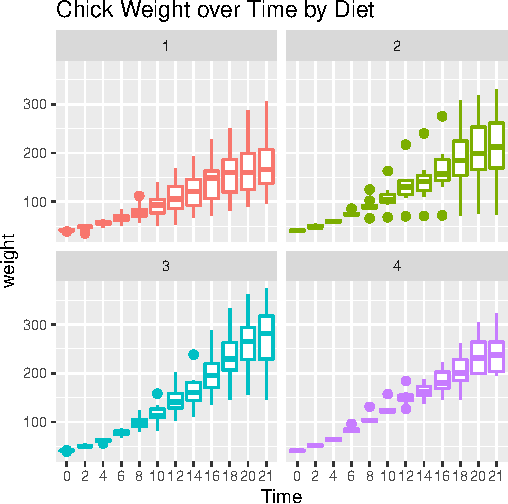
\includegraphics{Getting-Started-in-R_files/figure-latex/boxPlot-1} \end{center}

\subsection{Interpretation}\label{interpretation-4}

Looking at the graphs above we can say that diet 3 seems to have the
most ``average'' weight gain but it has more variation than diet 4. We
will have to look at the summary statistics to confirm this.

\subsection{Exercise}\label{exercise-7}

Add the following information to the the above plot:

\begin{itemize}
\tightlist
\item
  x-axis label (use \texttt{xlab()}): ``Time (days)''
\item
  y-axis label (use \texttt{ylab()}): ``Weight (grams)''
\end{itemize}

\subsection{Final Plot}\label{final-plot}

Let's finish with a plot that you might include in a publication.

\begin{Shaded}
\begin{Highlighting}[]
\KeywordTok{ggplot}\NormalTok{(CW, }\KeywordTok{aes}\NormalTok{(Time, weight, }\DataTypeTok{group=}\NormalTok{Diet, }
                             \DataTypeTok{colour=}\NormalTok{Diet)) }\OperatorTok{+}
\StringTok{  }\KeywordTok{facet_wrap}\NormalTok{(}\OperatorTok{~}\NormalTok{Diet) }\OperatorTok{+}
\StringTok{  }\KeywordTok{geom_jitter}\NormalTok{() }\OperatorTok{+}
\StringTok{  }\KeywordTok{stat_summary}\NormalTok{(}\DataTypeTok{fun.y=}\StringTok{"mean"}\NormalTok{, }\DataTypeTok{geom=}\StringTok{"line"}\NormalTok{,}
               \DataTypeTok{colour=}\StringTok{"black"}\NormalTok{) }\OperatorTok{+}
\StringTok{  }\KeywordTok{theme}\NormalTok{(}\DataTypeTok{legend.position =} \StringTok{"none"}\NormalTok{) }\OperatorTok{+}
\StringTok{  }\KeywordTok{ggtitle}\NormalTok{(}\StringTok{"Chick Weight over Time by Diet"}\NormalTok{) }\OperatorTok{+}\StringTok{ }
\StringTok{  }\KeywordTok{xlab}\NormalTok{(}\StringTok{"Time (days)"}\NormalTok{) }\OperatorTok{+}
\StringTok{  }\KeywordTok{ylab}\NormalTok{(}\StringTok{"Weight (grams)"}\NormalTok{)}
\end{Highlighting}
\end{Shaded}

\begin{center}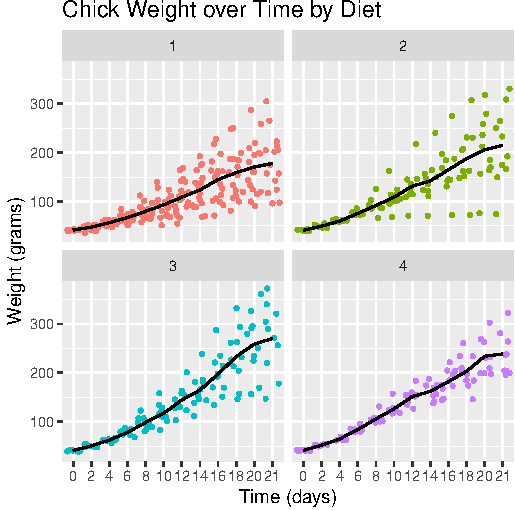
\includegraphics{Getting-Started-in-R_files/figure-latex/finalPlot-1} \end{center}

\section{Tidyverse: Data Wrangling
Basics}\label{tidyverse-data-wrangling-basics}

In this section we will learn how to wrangle (manipulate) datasets using
the \texttt{tidyverse} package. Let's start with the \texttt{mutate()},
\texttt{select()}, \texttt{rename()}, \texttt{filter()} and
\texttt{arrange()} functions.

\subsection{\texorpdfstring{\texttt{mutate()}}{mutate()}}\label{mutate}

Adds a new variable (column) or modifies an existing one. We already
used this above to create factor variables.

\begin{Shaded}
\begin{Highlighting}[]
\CommentTok{# Added a column}
\NormalTok{CWm1 <-}\StringTok{ }\KeywordTok{mutate}\NormalTok{(CW, }\DataTypeTok{weightKg =}\NormalTok{ weight}\OperatorTok{/}\DecValTok{1000}\NormalTok{)}
\NormalTok{CWm1}
\end{Highlighting}
\end{Shaded}

\begin{ShadedResult}
\begin{verbatim}
#  # A tibble: 578 x 5
#    Chick Diet  Time  weight weightKg
#    <dbl> <fct> <fct>  <dbl>    <dbl>
#  1    18 1     0         39    0.039
#  2    18 1     2         35    0.035
#  3    16 1     0         41    0.041
#  # ... with 575 more rows
\end{verbatim}
\end{ShadedResult}

\begin{Shaded}
\begin{Highlighting}[]
\CommentTok{# Modify an existing column}
\NormalTok{CWm2 <-}\StringTok{ }\KeywordTok{mutate}\NormalTok{(CW, }\DataTypeTok{Diet =} \KeywordTok{str_c}\NormalTok{(}\StringTok{"Diet "}\NormalTok{, Diet))}
\NormalTok{CWm2}
\end{Highlighting}
\end{Shaded}

\begin{ShadedResult}
\begin{verbatim}
#  # A tibble: 578 x 4
#    Chick Diet   Time  weight
#    <dbl> <chr>  <fct>  <dbl>
#  1    18 Diet 1 0         39
#  2    18 Diet 1 2         35
#  3    16 Diet 1 0         41
#  # ... with 575 more rows
\end{verbatim}
\end{ShadedResult}

\subsection{\texorpdfstring{\texttt{select()}}{select()}}\label{select}

Keeps, drops or reorders variables.

\begin{Shaded}
\begin{Highlighting}[]
\CommentTok{# Drop the weight variable from CWm1 using minus}
\KeywordTok{select}\NormalTok{(CWm1, }\OperatorTok{-}\NormalTok{weight)}
\end{Highlighting}
\end{Shaded}

\begin{ShadedResult}
\begin{verbatim}
#  # A tibble: 578 x 4
#    Chick Diet  Time  weightKg
#    <dbl> <fct> <fct>    <dbl>
#  1    18 1     0        0.039
#  2    18 1     2        0.035
#  3    16 1     0        0.041
#  # ... with 575 more rows
\end{verbatim}
\end{ShadedResult}

\begin{Shaded}
\begin{Highlighting}[]
\CommentTok{# Keep variables Time, Diet and weightKg}
\KeywordTok{select}\NormalTok{(CWm1, Chick, Time, Diet, weightKg)}
\end{Highlighting}
\end{Shaded}

\begin{ShadedResult}
\begin{verbatim}
#  # A tibble: 578 x 4
#    Chick Time  Diet  weightKg
#    <dbl> <fct> <fct>    <dbl>
#  1    18 0     1        0.039
#  2    18 2     1        0.035
#  3    16 0     1        0.041
#  # ... with 575 more rows
\end{verbatim}
\end{ShadedResult}

\subsection{\texorpdfstring{\texttt{rename()}}{rename()}}\label{rename}

Renames variables whilst keeping all variables.

\begin{Shaded}
\begin{Highlighting}[]
\KeywordTok{rename}\NormalTok{(CW, }\DataTypeTok{Group =}\NormalTok{ Diet, }\DataTypeTok{Weight =}\NormalTok{ weight)}
\end{Highlighting}
\end{Shaded}

\begin{ShadedResult}
\begin{verbatim}
#  # A tibble: 578 x 4
#    Chick Group Time  Weight
#    <dbl> <fct> <fct>  <dbl>
#  1    18 1     0         39
#  2    18 1     2         35
#  3    16 1     0         41
#  # ... with 575 more rows
\end{verbatim}
\end{ShadedResult}

\subsection{\texorpdfstring{\texttt{filter()}}{filter()}}\label{filter}

Keeps or drops observations (rows).

\begin{Shaded}
\begin{Highlighting}[]
\KeywordTok{filter}\NormalTok{(CW, Time}\OperatorTok{==}\DecValTok{21} \OperatorTok{&}\StringTok{ }\NormalTok{weight}\OperatorTok{>}\DecValTok{300}\NormalTok{)}
\end{Highlighting}
\end{Shaded}

\begin{ShadedResult}
\begin{verbatim}
#  # A tibble: 8 x 4
#    Chick Diet  Time  weight
#    <dbl> <fct> <fct>  <dbl>
#  1     7 1     21       305
#  2    29 2     21       309
#  3    21 2     21       331
#  # ... with 5 more rows
\end{verbatim}
\end{ShadedResult}

For comparing values in vectors use: \texttt{\textless{}} (less than),
\texttt{\textgreater{}} (greater than), \texttt{\textless{}=} (less than
and equal to), \texttt{\textgreater{}=} (greater than and equal to),
\texttt{==} (equal to) and \texttt{!=} (not equal to). These can be
combined logically using \texttt{\&} (and) and \texttt{\textbar{}} (or).

\subsection{\texorpdfstring{\texttt{arrange()}}{arrange()}}\label{arrange}

Changes the order of the observations (rows).

\begin{Shaded}
\begin{Highlighting}[]
\KeywordTok{arrange}\NormalTok{(CW, Chick, Time)}
\end{Highlighting}
\end{Shaded}

\begin{ShadedResult}
\begin{verbatim}
#  # A tibble: 578 x 4
#    Chick Diet  Time  weight
#    <dbl> <fct> <fct>  <dbl>
#  1     1 1     0         42
#  2     1 1     2         51
#  3     1 1     4         59
#  # ... with 575 more rows
\end{verbatim}
\end{ShadedResult}

\begin{Shaded}
\begin{Highlighting}[]
\KeywordTok{arrange}\NormalTok{(CW, }\KeywordTok{desc}\NormalTok{(weight))}
\end{Highlighting}
\end{Shaded}

\begin{ShadedResult}
\begin{verbatim}
#  # A tibble: 578 x 4
#    Chick Diet  Time  weight
#    <dbl> <fct> <fct>  <dbl>
#  1    35 3     21       373
#  2    35 3     20       361
#  3    34 3     21       341
#  # ... with 575 more rows
\end{verbatim}
\end{ShadedResult}

\subsection{Exercise}\label{exercise-8}

What does the \texttt{desc()} do? Try using \texttt{desc(Time)}.

\section{\texorpdfstring{Tidyverse: Pipe operator
\texttt{\%\textgreater{}\%}}{Tidyverse: Pipe operator \%\textgreater{}\%}}\label{tidyverse-pipe-operator}

In reality you will end up doing multiple data wrangling steps that you
want to save. Neither are optimal as they have their own issues. This is
where the pipe operator, \texttt{\%\textgreater{}\%} comes to the
rescue:

\begin{Shaded}
\begin{Highlighting}[]
\NormalTok{CW21 <-}\StringTok{ }\NormalTok{CW }\OperatorTok\StringTok{ }
\StringTok{  }\KeywordTok{filter}\NormalTok{(Time }\OperatorTok\StringTok{ }\KeywordTok{c}\NormalTok{(}\DecValTok{0}\NormalTok{, }\DecValTok{21}\NormalTok{)) }\OperatorTok\StringTok{ }
\StringTok{  }\KeywordTok{rename}\NormalTok{(}\DataTypeTok{Weight =}\NormalTok{ weight) }\OperatorTok\StringTok{ }
\StringTok{  }\KeywordTok{mutate}\NormalTok{(}\DataTypeTok{Group =} \KeywordTok{factor}\NormalTok{(}\KeywordTok{str_c}\NormalTok{(}\StringTok{"Diet "}\NormalTok{, Diet))) }\OperatorTok\StringTok{ }
\StringTok{  }\KeywordTok{select}\NormalTok{(Chick, Group, Time, Weight) }\OperatorTok\StringTok{ }
\StringTok{  }\KeywordTok{arrange}\NormalTok{(Chick, Time) }
\NormalTok{CW21}
\end{Highlighting}
\end{Shaded}

\begin{ShadedResult}
\begin{verbatim}
#  # A tibble: 95 x 4
#    Chick Group  Time  Weight
#    <dbl> <fct>  <fct>  <dbl>
#  1     1 Diet 1 0         42
#  2     1 Diet 1 21       205
#  3     2 Diet 1 0         40
#  # ... with 92 more rows
\end{verbatim}
\end{ShadedResult}

\subsection{\texorpdfstring{Read \texttt{\%\textgreater{}\%} as
``then''}{Read \%\textgreater{}\% as then}}\label{read-as-then}

To understand the code above we should read the pipe operator
\texttt{\%\textgreater{}\%} as ``then''.

\begin{quote}
Create a new dataset (object) called \texttt{CW21} using dataset
\texttt{CW} \textbf{\emph{then}} keep the data for days 0 and 21
\textbf{\emph{then}} rename variable \texttt{weight} to \texttt{Weight}
\textbf{\emph{then}} create a variable called \texttt{Group}
\textbf{\emph{then}} keep variables \texttt{Chick}, \texttt{Group},
\texttt{Time} and \texttt{Weight} and \textbf{\emph{then}} finally
arrange the data by variables \texttt{Chick} and \texttt{Time}.
\end{quote}

\subsection{In practice}\label{in-practice}

\begin{Shaded}
\begin{Highlighting}[]
\NormalTok{CW21 <-}\StringTok{ }\NormalTok{CW }\OperatorTok\StringTok{ }
\StringTok{  }\KeywordTok{filter}\NormalTok{(., Time }\OperatorTok\StringTok{ }\KeywordTok{c}\NormalTok{(}\DecValTok{0}\NormalTok{, }\DecValTok{21}\NormalTok{)) }\OperatorTok\StringTok{ }
\StringTok{  }\KeywordTok{rename}\NormalTok{(., }\DataTypeTok{Weight =}\NormalTok{ weight) }\OperatorTok\StringTok{ }
\StringTok{  }\KeywordTok{mutate}\NormalTok{(., }\DataTypeTok{Group=}\KeywordTok{factor}\NormalTok{(}\KeywordTok{str_c}\NormalTok{(}\StringTok{"Diet "}\NormalTok{,Diet))) }\OperatorTok\StringTok{ }
\StringTok{  }\KeywordTok{select}\NormalTok{(., Chick, Group, Time, Weight) }\OperatorTok\StringTok{ }
\StringTok{  }\KeywordTok{arrange}\NormalTok{(., Chick, Time) }
\end{Highlighting}
\end{Shaded}

The pipe operator, \texttt{\%\textgreater{}\%}, replaces the dots
(\texttt{.}) with whatever is returned from code preceding it. For
example, the dot in \texttt{filter(.,\ Time\ \%in\%\ c(0,\ 21))} is
replaced by \texttt{CW}. The output of the \texttt{filter(...)} then
replaces the dot in \texttt{rename(.,\ Weight\ =\ weight)} and so on.
Think of it as a data assembly line with each function doing its thing
and passing it to the next.

\section{Chick Weight: Summary
Statistics}\label{chick-weight-summary-statistics}

Having done some data visualisations we will quantify the effects of the
diets using summmary statistics. First we will look at the number of
observations and the mean by diet and time.

\begin{Shaded}
\begin{Highlighting}[]
\NormalTok{mnsdCW <-}\StringTok{ }\NormalTok{CW }\OperatorTok\StringTok{ }
\StringTok{  }\KeywordTok{group_by}\NormalTok{(Diet, Time) }\OperatorTok\StringTok{ }
\StringTok{  }\KeywordTok{summarise}\NormalTok{(}\DataTypeTok{N =} \KeywordTok{n}\NormalTok{(), }\DataTypeTok{Mean =} \KeywordTok{mean}\NormalTok{(weight)) }\OperatorTok\StringTok{ }
\StringTok{  }\KeywordTok{arrange}\NormalTok{(Diet, Time)}
\NormalTok{mnsdCW}
\end{Highlighting}
\end{Shaded}

\begin{ShadedResult}
\begin{verbatim}
#  # A tibble: 48 x 4
#  # Groups:   Diet [4]
#    Diet  Time      N  Mean
#    <fct> <fct> <int> <dbl>
#  1 1     0        20  41.4
#  2 1     2        20  47.2
#  3 1     4        19  56.5
#  # ... with 45 more rows
\end{verbatim}
\end{ShadedResult}

For each distinct combination of \texttt{Diet} and \texttt{Time}, the
chick weight data is summarised into the number of observations
(\texttt{N}) and the mean (\texttt{Mean}) of \texttt{weight}.

Let's also calculate the standard deviation, median, minimum and maximum
values but only at days 0 (zero) and 21.

\begin{Shaded}
\begin{Highlighting}[]
\NormalTok{sumCW <-}\StringTok{  }\NormalTok{CW }\OperatorTok\StringTok{ }
\StringTok{  }\KeywordTok{filter}\NormalTok{(Time }\OperatorTok\StringTok{ }\KeywordTok{c}\NormalTok{(}\DecValTok{0}\NormalTok{, }\DecValTok{21}\NormalTok{)) }\OperatorTok\StringTok{ }
\StringTok{  }\KeywordTok{group_by}\NormalTok{(Diet, Time) }\OperatorTok\StringTok{ }
\StringTok{  }\KeywordTok{summarise}\NormalTok{(}\DataTypeTok{N =} \KeywordTok{n}\NormalTok{(),}
            \DataTypeTok{Mean =} \KeywordTok{mean}\NormalTok{(weight),}
            \DataTypeTok{SD =} \KeywordTok{sd}\NormalTok{(weight),}
            \DataTypeTok{Median =} \KeywordTok{median}\NormalTok{(weight),}
            \DataTypeTok{Min =} \KeywordTok{min}\NormalTok{(weight),}
            \DataTypeTok{Max =} \KeywordTok{max}\NormalTok{(weight)) }\OperatorTok\StringTok{ }
\StringTok{  }\KeywordTok{arrange}\NormalTok{(Diet, Time)}
\NormalTok{sumCW}
\end{Highlighting}
\end{Shaded}

\begin{ShadedResult}
\begin{verbatim}
#  # A tibble: 8 x 8
#  # Groups:   Diet [4]
#    Diet  Time      N  Mean     SD Median   Min
#    <fct> <fct> <int> <dbl>  <dbl>  <dbl> <dbl>
#  1 1     0        20  41.4  0.995   41      39
#  2 1     21       16 178.  58.7    166      96
#  3 2     0        10  40.7  1.49    40.5    39
#  # ... with 5 more rows, and 1 more variable:
#  #   Max <dbl>
\end{verbatim}
\end{ShadedResult}

Let's make the summaries ``prettier'', say, for a report or publication.

\begin{Shaded}
\begin{Highlighting}[]
\NormalTok{prettySumCW <-}\StringTok{ }\NormalTok{sumCW }\OperatorTok\StringTok{ }
\StringTok{ }\KeywordTok{mutate}\NormalTok{(}\DataTypeTok{Mean_SD =} \KeywordTok{str_c}\NormalTok{(}\KeywordTok{format}\NormalTok{(Mean, }\DataTypeTok{digits=}\DecValTok{1}\NormalTok{),}
           \StringTok{" ("}\NormalTok{, }\KeywordTok{format}\NormalTok{(SD, }\DataTypeTok{digits=}\DecValTok{2}\NormalTok{), }\StringTok{")"}\NormalTok{)) }\OperatorTok\StringTok{ }
\StringTok{ }\KeywordTok{mutate}\NormalTok{(}\DataTypeTok{Range =} \KeywordTok{str_c}\NormalTok{(Min, }\StringTok{" - "}\NormalTok{, Max)) }\OperatorTok\StringTok{ }
\StringTok{ }\KeywordTok{select}\NormalTok{(Diet, Time, N, Mean_SD, Median, Range) }\OperatorTok
\StringTok{ }\KeywordTok{arrange}\NormalTok{(Diet, Time)}
\NormalTok{prettySumCW}
\end{Highlighting}
\end{Shaded}

\begin{ShadedResult}
\begin{verbatim}
#  # A tibble: 8 x 6
#  # Groups:   Diet [4]
#    Diet  Time      N Mean_SD    Median Range 
#    <fct> <fct> <int> <chr>       <dbl> <chr> 
#  1 1     0        20 " 41 ( 0.~   41   39 - ~
#  2 1     21       16 178 (58.7~  166   96 - ~
#  3 2     0        10 " 41 ( 1.~   40.5 39 - ~
#  # ... with 5 more rows
\end{verbatim}
\end{ShadedResult}

\subsection{Final Table}\label{final-table}

Eventually you should be able to produce\footnote{Using the
  \texttt{kable()} function from the \texttt{knitr} package with
  functions from the \texttt{kableExtra} package.} a publication ready
version as follows:

\begin{table}[H]
\centering
\begin{tabular}{cccrccccrccccrccccrccccrccccrc}
\toprule
\textbf{Diet} & \textbf{Time} & \textbf{N} & \textbf{Mean\_SD} & \textbf{Median} & \textbf{Range}\\
\midrule
1 & 0 & 20 & 41 ( 0.99) & 41.0 & 39 - 43\\
\rowcolor{lightgray}  1 & 21 & 16 & 178 (58.70) & 166.0 & 96 - 305\\
2 & 0 & 10 & 41 ( 1.5) & 40.5 & 39 - 43\\
\rowcolor{lightgray}  2 & 21 & 10 & 215 (78.1) & 212.5 & 74 - 331\\
3 & 0 & 10 & 41 ( 1) & 41.0 & 39 - 42\\
\rowcolor{lightgray}  3 & 21 & 10 & 270 (72) & 281.0 & 147 - 373\\
4 & 0 & 10 & 41 ( 1.1) & 41.0 & 39 - 42\\
\rowcolor{lightgray}  4 & 21 & 9 & 239 (43.3) & 237.0 & 196 - 322\\
\bottomrule
\end{tabular}
\end{table}

\subsection{Interpretation}\label{interpretation-5}

This summary table offers the same interpretation as before, namely that
diet 3 has the highest mean and median weights at day 21 but a higher
variation than group 4. However it should be noted that at day 21, diet
1 lost 4 chicks from 20 that started and diet 4 lost 1 from 10. This
could be a sign of some issues (e.g.~safety).

\subsection{Limitations of data}\label{limitations-of-data}

Information on bias reduction measures is not given and is not available
either\footnote{I contacted the source authors and kindly received the
  following reply \emph{``They were mainly undergraduate projects,
  final-year, rather than theses, so, unfortunately, it's unlikely that
  any record remains, particularly after so many years.''}}. We don't
know if the chicks were fairly and appropriately randomised to the diets
and whether the groups are compariable (e.g., same breed of chicks, sex
(gender) balance). Hence we should be very cautious with drawing
conclusion and taking actions with this data.

\section{Conclusion}\label{conclusion}

This ``Getting Started in R'' guide introduced you to some of the basic
concepts underlying R and used a real life dataset to produce some
graphs and summary statistics. It is only a flavour of what R can do but
hopefully you have seen some of power of R and its potential.

\subsection{What next}\label{what-next}

There are plenty of R courses, books and on-line resources that you can
learn from. It is hard to recommend any in particular as it depends on
how you learn best. Find things that work for you (paying attention to
the quality) and don't be afraid to make mistakes or ask questions. Most
importantly have fun.

%\showmatmethods
\showacknow





\end{document}

